%Title: Mugast-Comissioning Analysis Report- slide back
%Author: A. Raggio
%Year: 2019

\documentclass[10pt]{beamer}

%
%Setting file
%

\usepackage[T1]{fontenc}
\usepackage[utf8]{inputenc}

\usepackage[english]{babel}

\usepackage{graphicx}
\graphicspath{{images/}}
\usepackage{float}
\usepackage{tikz}
\usepackage{caption}
\usepackage{subcaption}

\usetheme{Ilmenau}
\usecolortheme{lily}
\usefonttheme{structurebold}

\setbeamertemplate{itemize items}[circle]

\setbeamertemplate{title page}
{
  \begin{centering}
     {\usebeamercolor[fg]{titlegraphic}\center\inserttitlegraphic\par}
    \begin{beamercolorbox}[sep=15pt,center]{institute}
      \usebeamerfont{institute}\insertinstitute
    \end{beamercolorbox}
    \begin{beamercolorbox}[sep=8pt,center,rounded=true]{title}
      \usebeamerfont{title}\inserttitle\par%
      \ifx\insertsubtitle\@empty%
      \else%
        \vskip0.25em%
        {\usebeamerfont{subtitle}\usebeamercolor[fg]{subtitle}\insertsubtitle\par}%
      \fi%     
    \end{beamercolorbox}%
    \begin{beamercolorbox}[sep=20pt,center]{author}
      \usebeamerfont{author}\insertauthor
    \end{beamercolorbox}
   \end{centering}
  \vfill
}

\setbeamertemplate{frametitle}
{
    \nointerlineskip
    \begin{beamercolorbox}[sep=0.35cm,ht=2em,wd=\paperwidth]{frametitle}
		    
        \centering
        \insertframetitle
    \end{beamercolorbox}
}


\addtobeamertemplate{frametitle}{}{%
\begin{tikzpicture}[remember picture,overlay]
\node[anchor=north west,yshift=-22pt,xshift=-2pt] at (current page.north west) {\includegraphics[height=.10\textheight]{INFN_LOGO}};
\end{tikzpicture}} 


\beamertemplatenavigationsymbolsempty
\setbeamercovered{transparent}




\begin{document}
\begin{frame}
\centering
\vspace{-0.15\textheight}
\textbf{AGATA+MUGAST+VAMOS\\ COMMISSIONING}
\vspace{0.05\textheight}
\begin{columns}
	\begin{column}{0.5\textwidth}
		\begin{overlayarea}{\textwidth}{0.5\textheight}
			\center
			\text{\color{red}Commissioning Reaction}\\
			\vspace{0.02\textheight}
			\textbf{\large$\mathbf{^{16}}$O(d,p)$\mathbf{^{17}}$O}\\
			\vspace{0.02\textheight}
			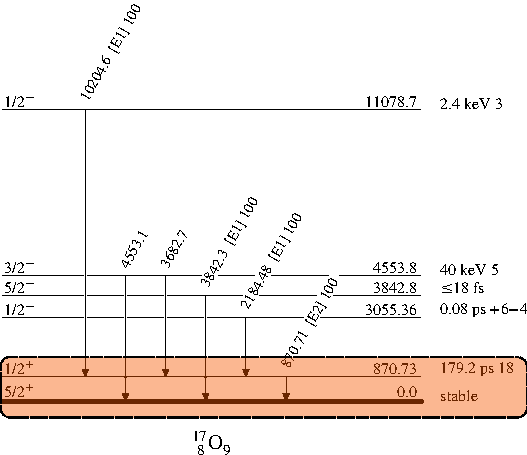
\includegraphics[width=\textwidth]{level_17O_1}
		\end{overlayarea}
	\end{column}
	\begin{column}{0.5\textwidth}
		\begin{overlayarea}{\textwidth}{0.5\textheight}
			\center
			\text{\color{red}Preliminary Results}
			\vspace{0.05\textheight}
			\begin{itemize}
				\item[$\rightarrow$]Angular distribution for transfer to g.s. and 1/2+ of $\mathbf{^{17}}$O.
				\item[$\rightarrow$]Proton-gamma coincidence for the 870~keV gamma decay.
				\item[$\rightarrow$]AGATA efficiency estimate.
			\end{itemize}
		\end{overlayarea}
	\end{column}
\end{columns}

\end{frame}

\begin{frame}
\centering
\vspace{0.05\textheight}
\textbf{\LARGE Set Up}
\vspace{0.05\textheight}
\begin{columns}
	\begin{column}{0.6\textwidth}
			\centering
			\vspace{-0.1\textheight}
			\begin{columns}
				\begin{column}{0.5\textwidth}
					\center
					\textbf{BEAM}\\
					\vspace{0.03\textheight}
					$\mathbf{^{16}}$O \\
					6~MeV/u - $10^{4}$pps
				\end{column}
	
				\begin{column}{0.5\textwidth}
					\center
					\textbf{TARGET}\\
					\vspace{0.03\textheight}
					CD2\\
					1~mg/cm$^2$	
				\end{column}
			\end{columns}
			\vspace{0.05\textheight}
			\textbf{\Large Detectors}
			\vspace{0.03\textheight}
			\begin{columns}
				\begin{column}{0.5\textwidth}
					\centering\\
					\textbf{AGATA}\\
					\begin{itemize}
						\item 37 crystal
					\end{itemize}
					\vspace{0.03\textheight}
					\textbf{VAMOS}\\  
					\begin{itemize}
						\item MWPPAC
						\item Drift Chambers
						\item Ionization Chambers
					\end{itemize}
				\end{column}
	
				\begin{column}{0.5\textwidth}
					\centering\\
					\vspace{-0.04\textheight}
					\textbf{MUGAST}\\
					\begin{itemize}
						\item 5 trapezoidal DSSD
	 					\item 1 anular DSSD
	 					\item 2 square DSSD 
	 					\item 4 MUST2 Telescope
					\end{itemize}
				\end{column}
			\end{columns}

		
	\end{column}
	\begin{column}{0.4\textwidth}
		\vspace{-0.08\textheight}\\
		\hspace{0.4\textwidth}
		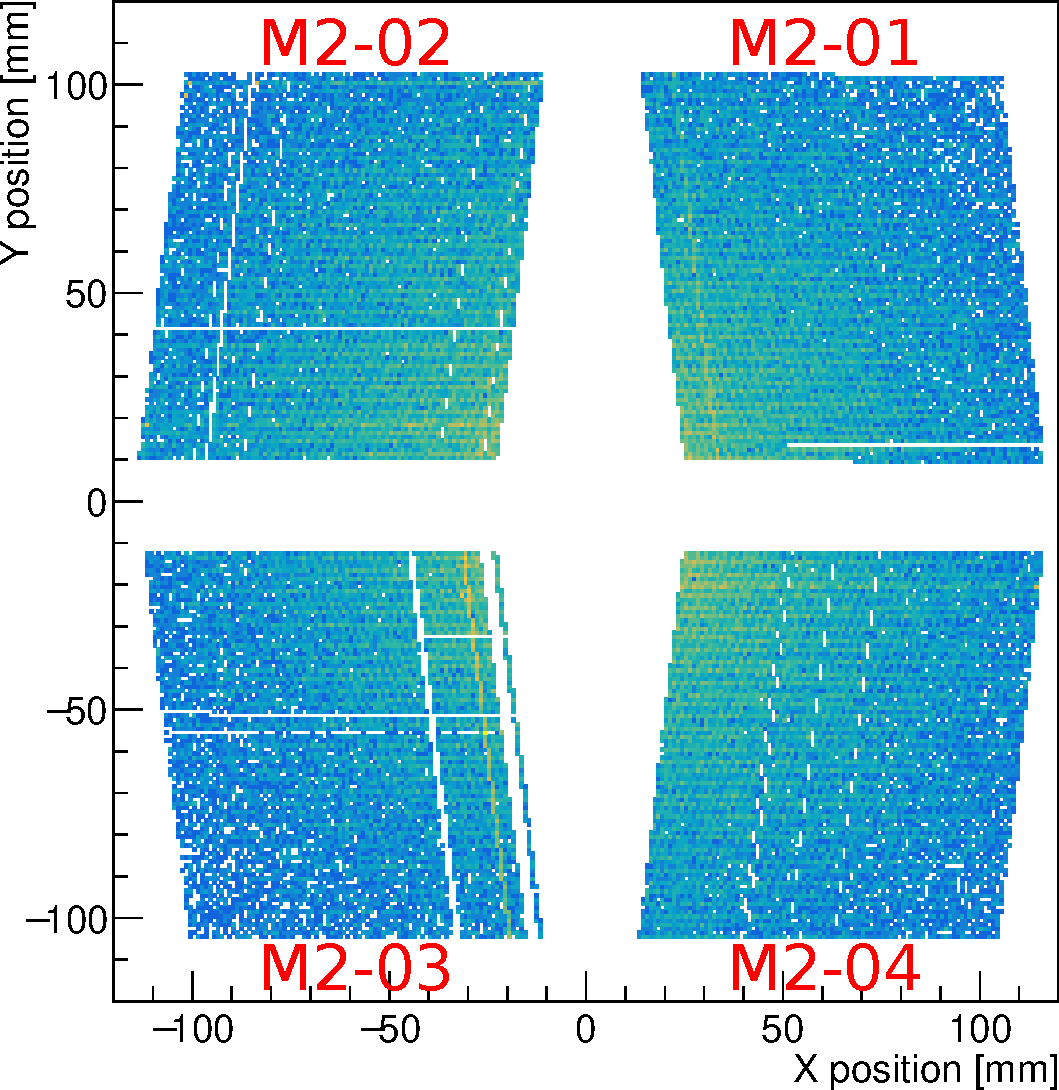
\includegraphics[height=0.3\textheight]{MMimpact}\\
		\hspace{0.\textwidth}
		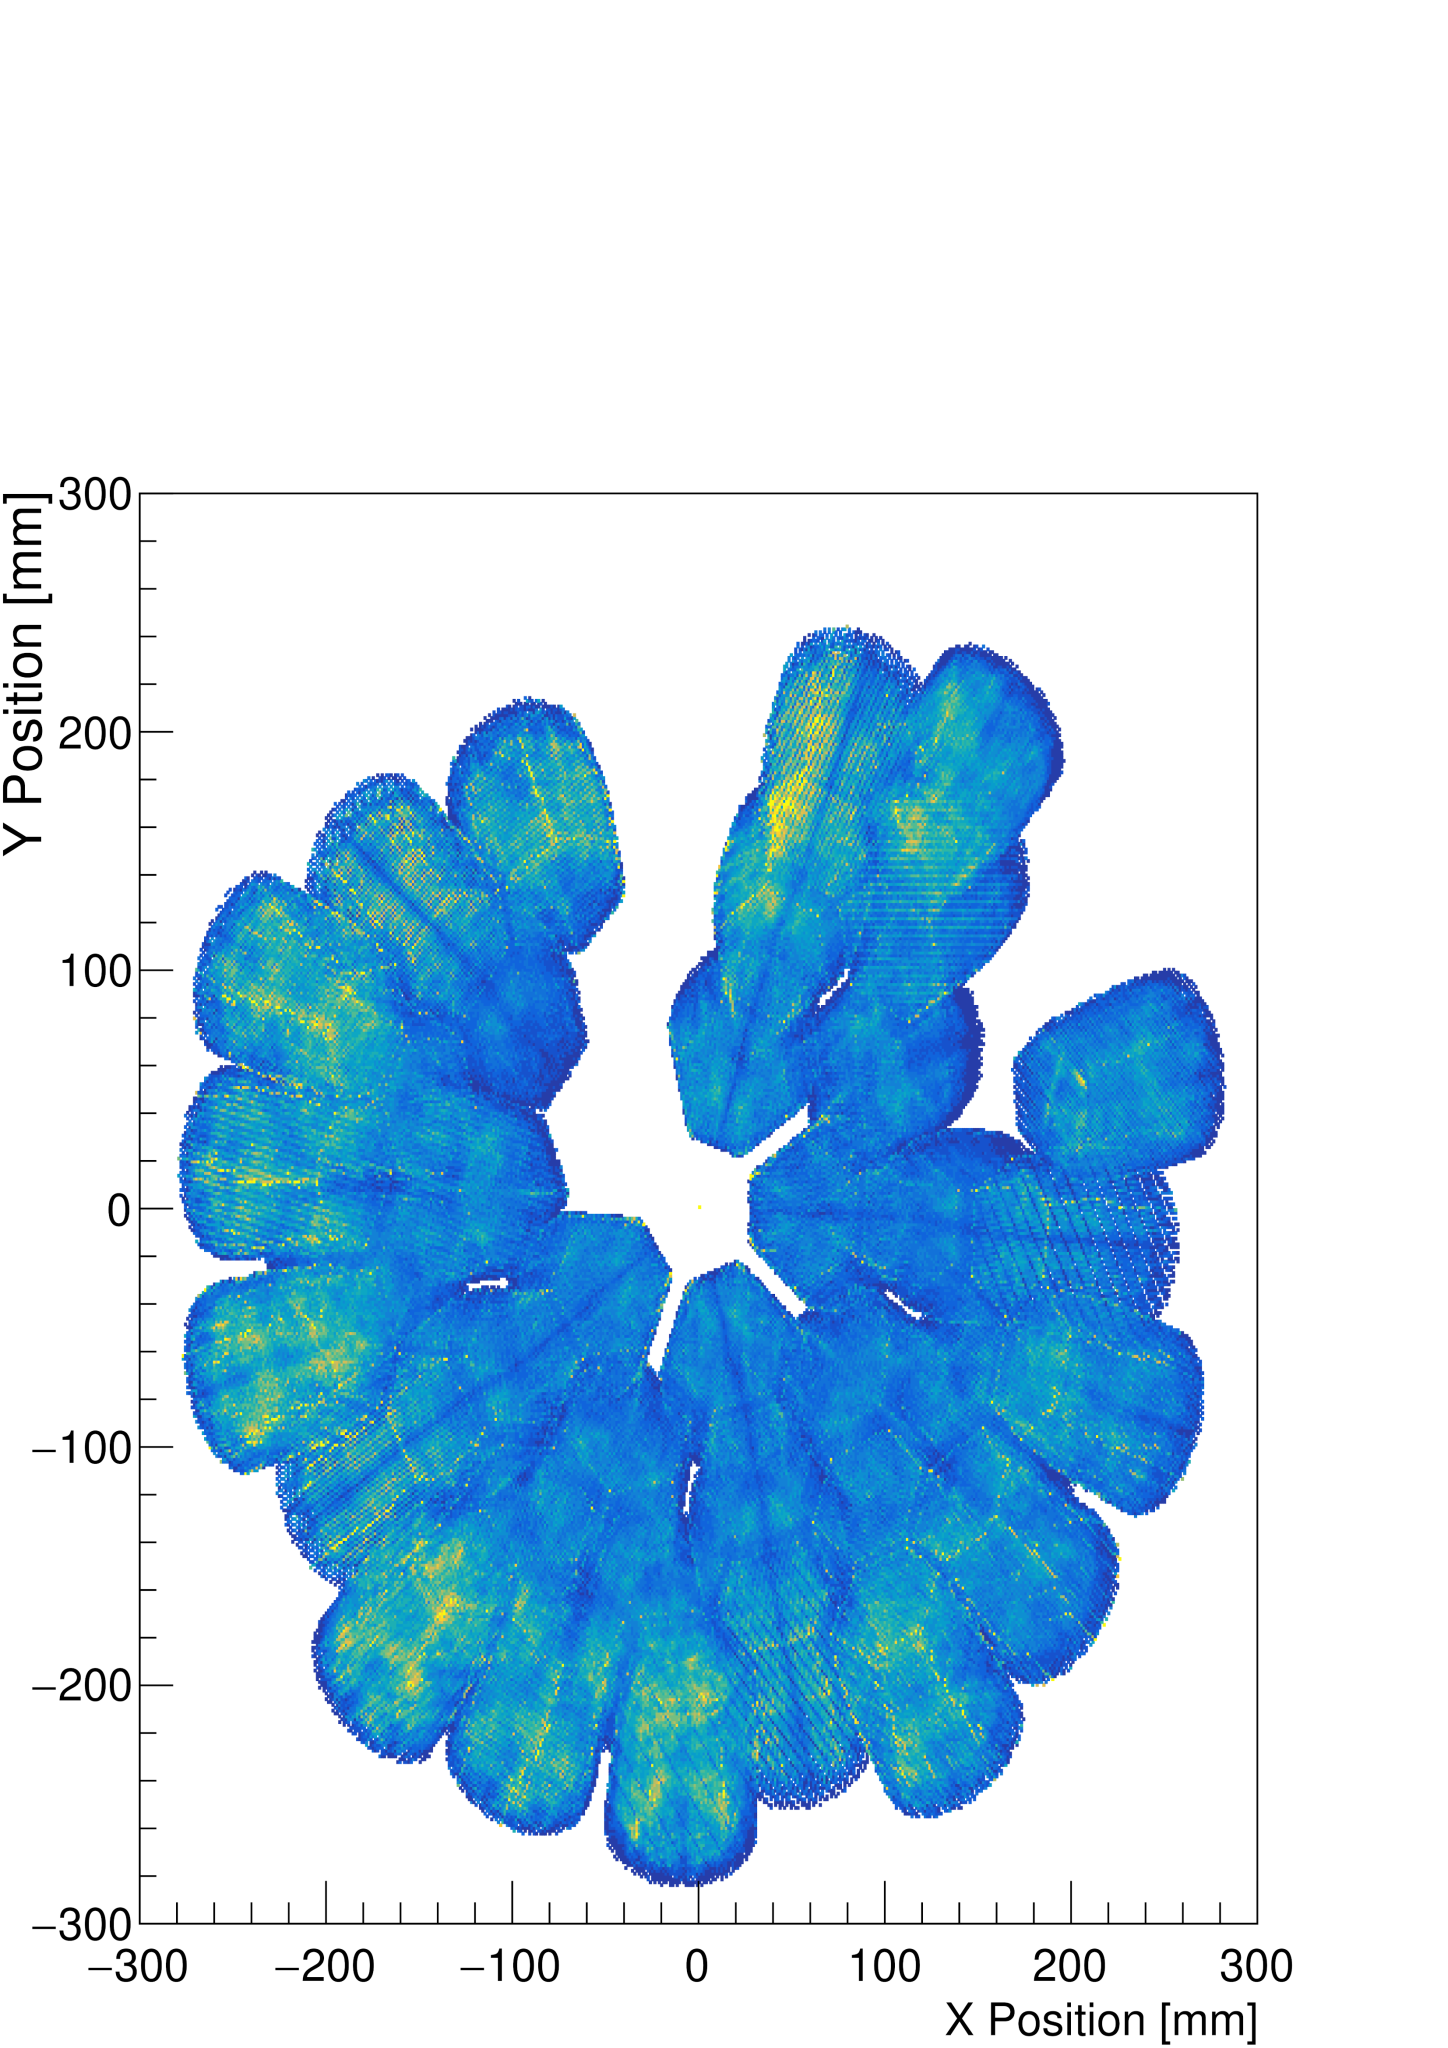
\includegraphics[height=0.3\textheight, width=0.57\textwidth]{AGATAimpact}\\
		\hspace{0.4\textwidth}
		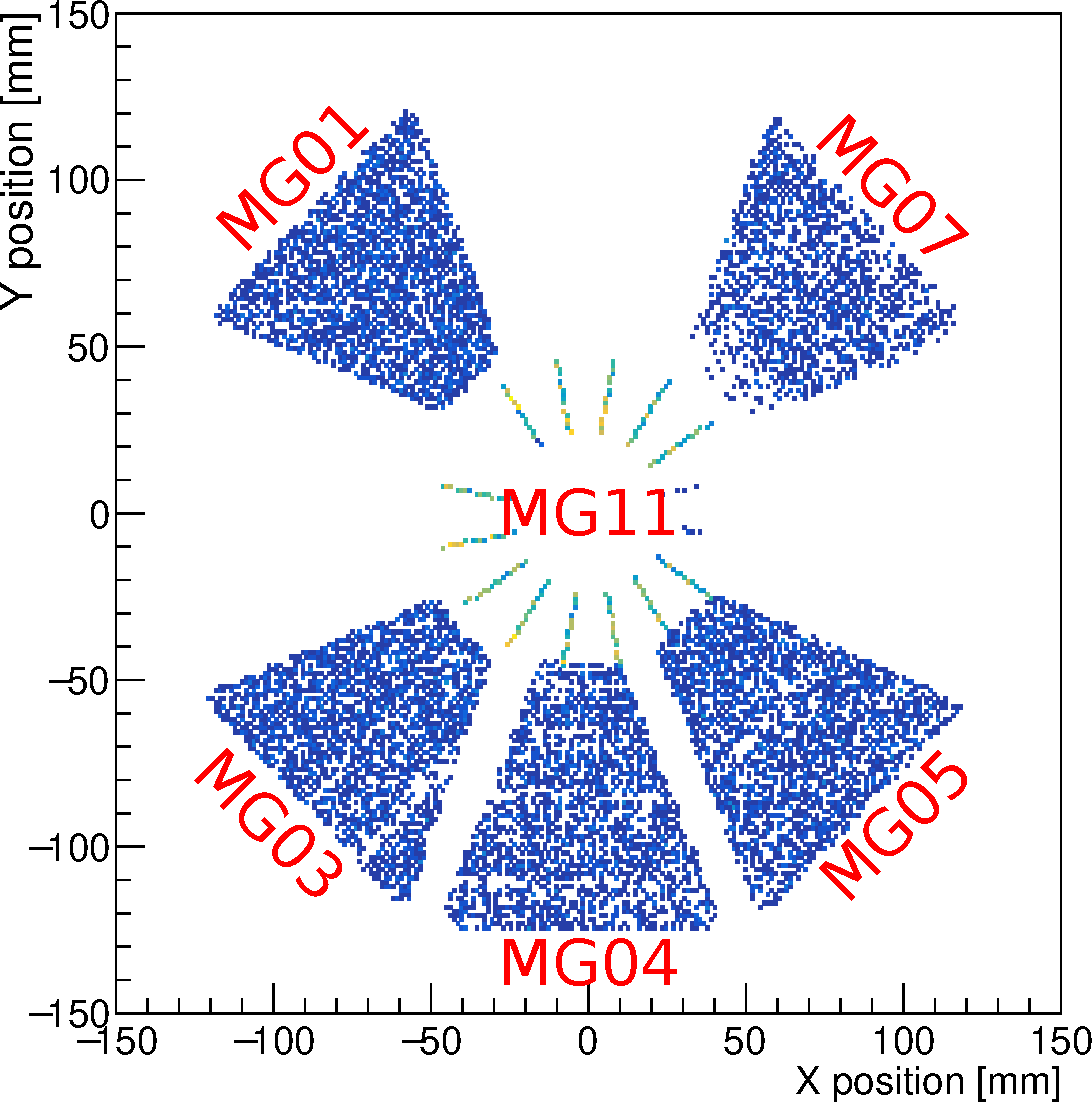
\includegraphics[height=0.3\textheight]{MGimpact}\\

	\end{column}
\end{columns}

\end{frame}

\begin{frame}
\centering
\vspace{0.03\textheight}
\textbf{\Large Kinematic Lines}
\vspace{0.01\textheight}
\begin{columns}
	\begin{column}{0.4\textwidth}
		\centering
		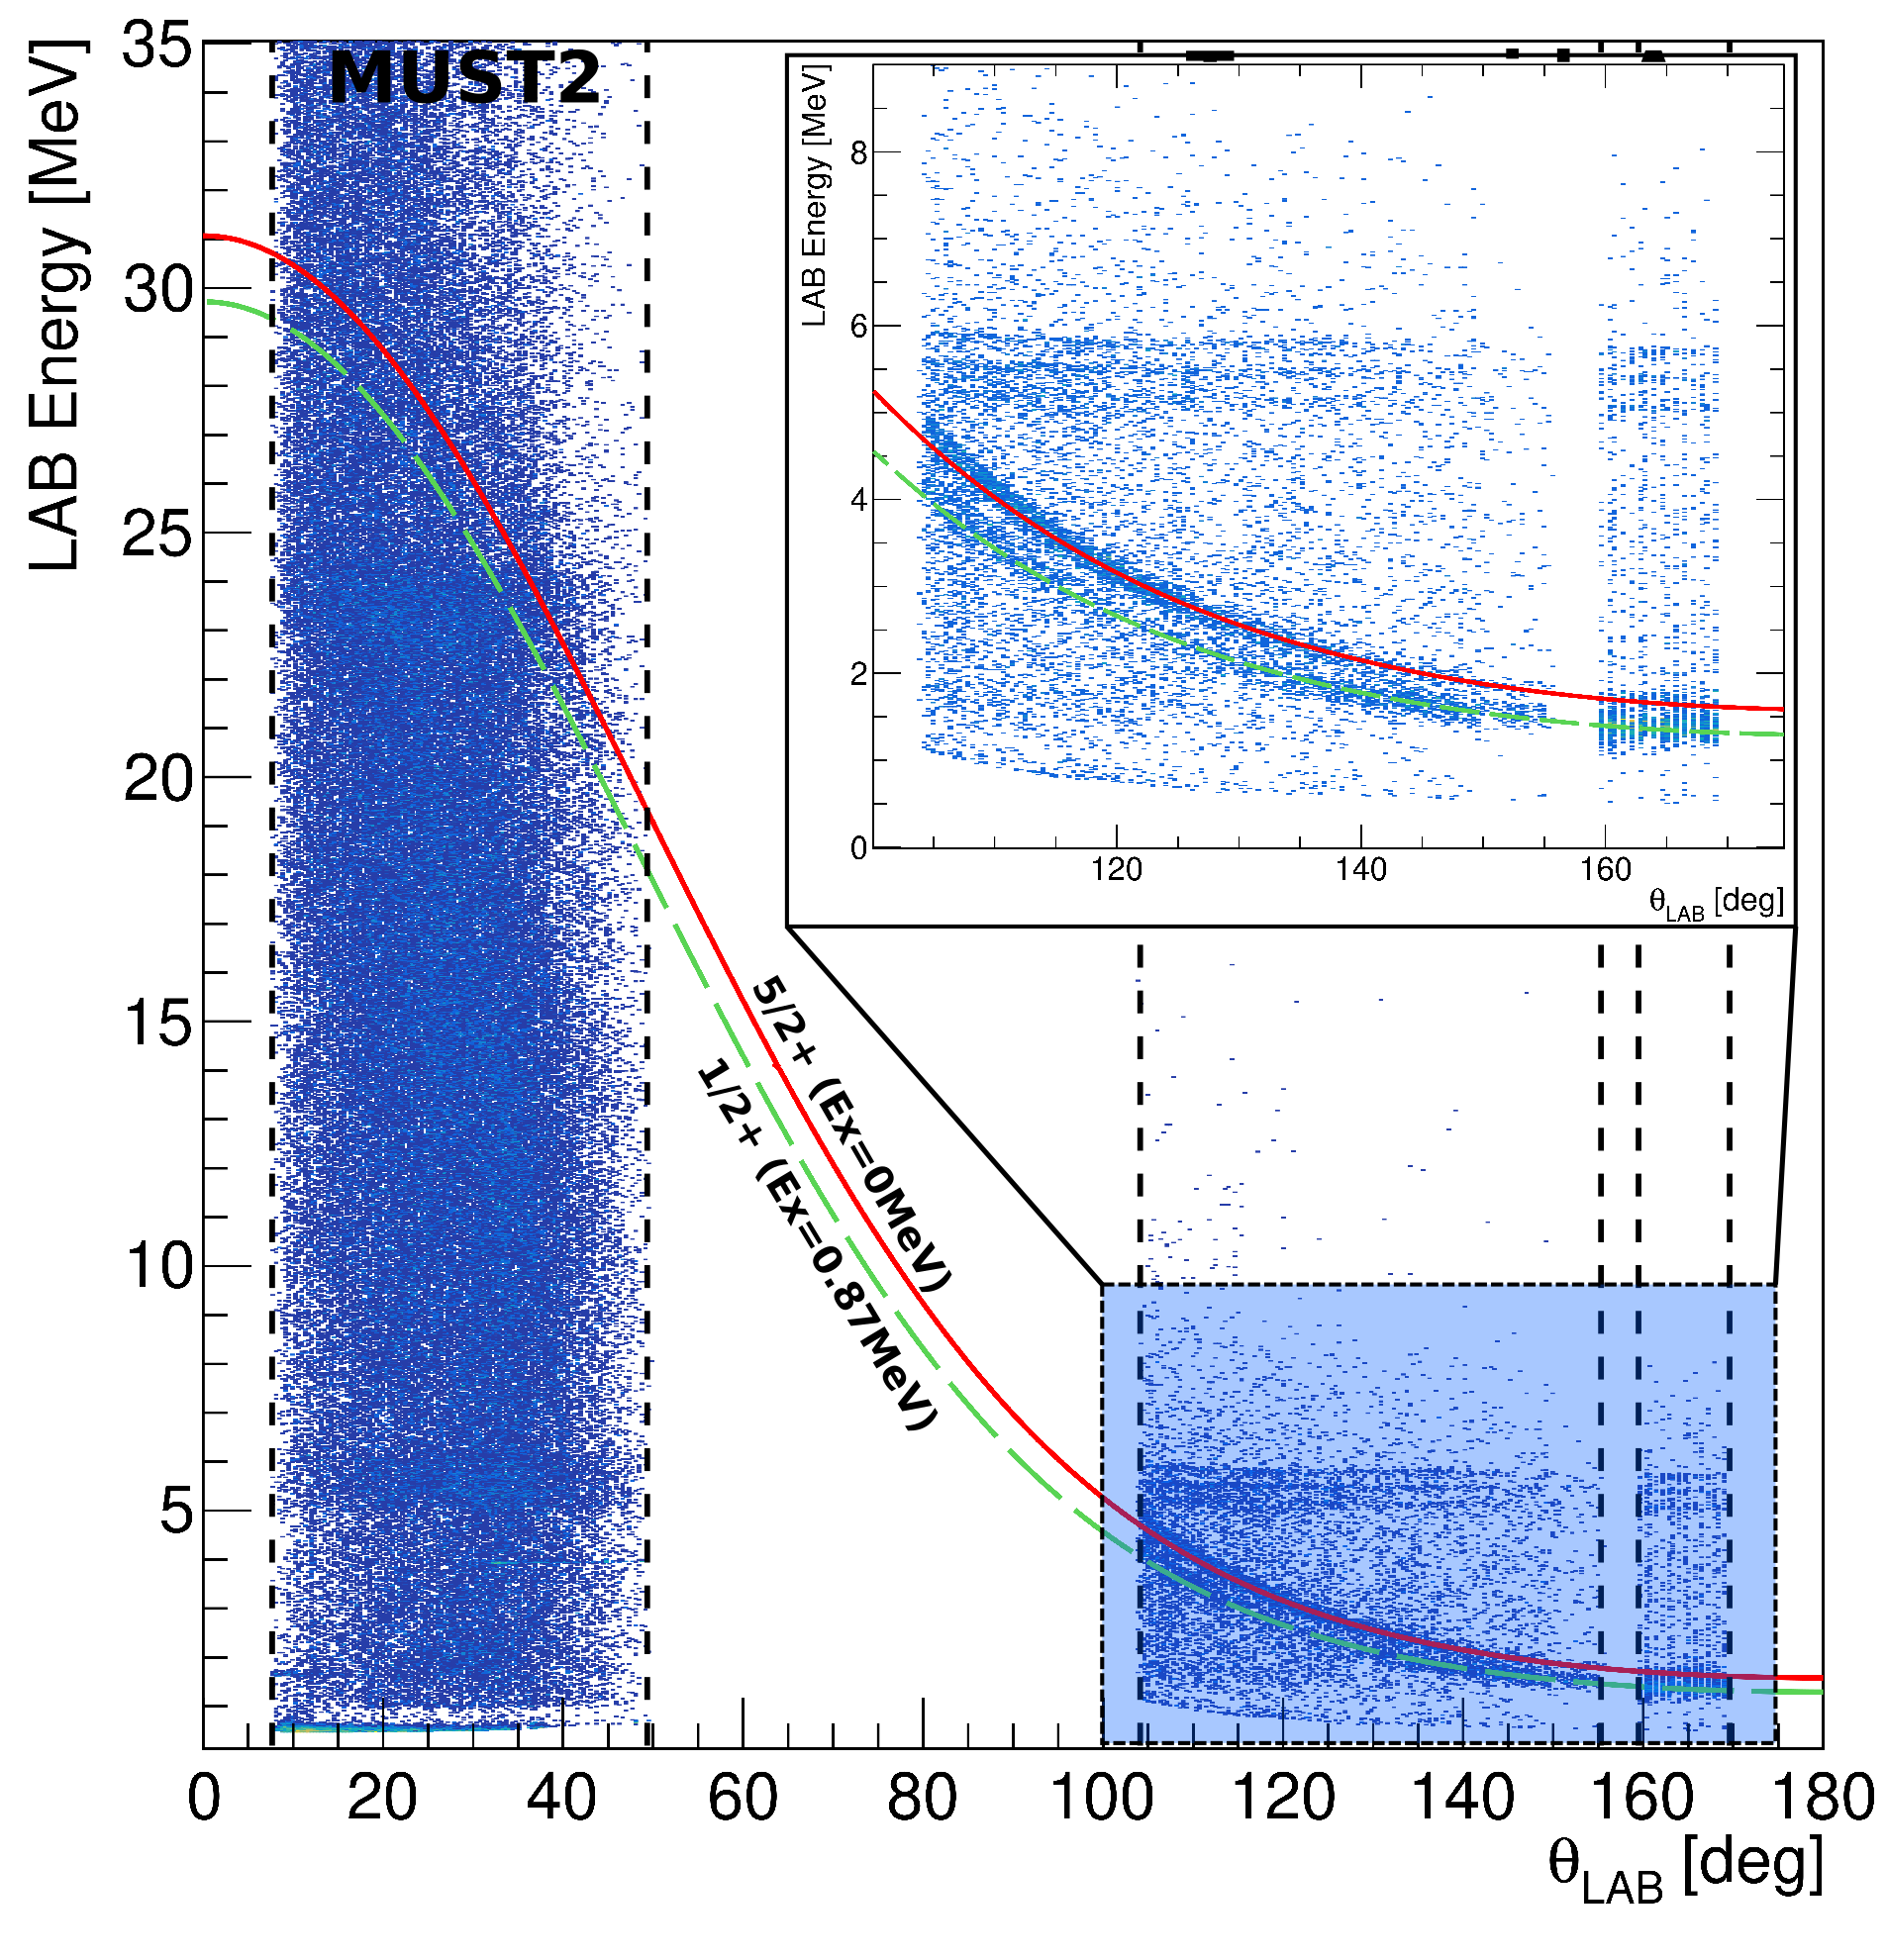
\includegraphics[width=0.9\textwidth]{ELabVsThetaLab_1.png}\\
		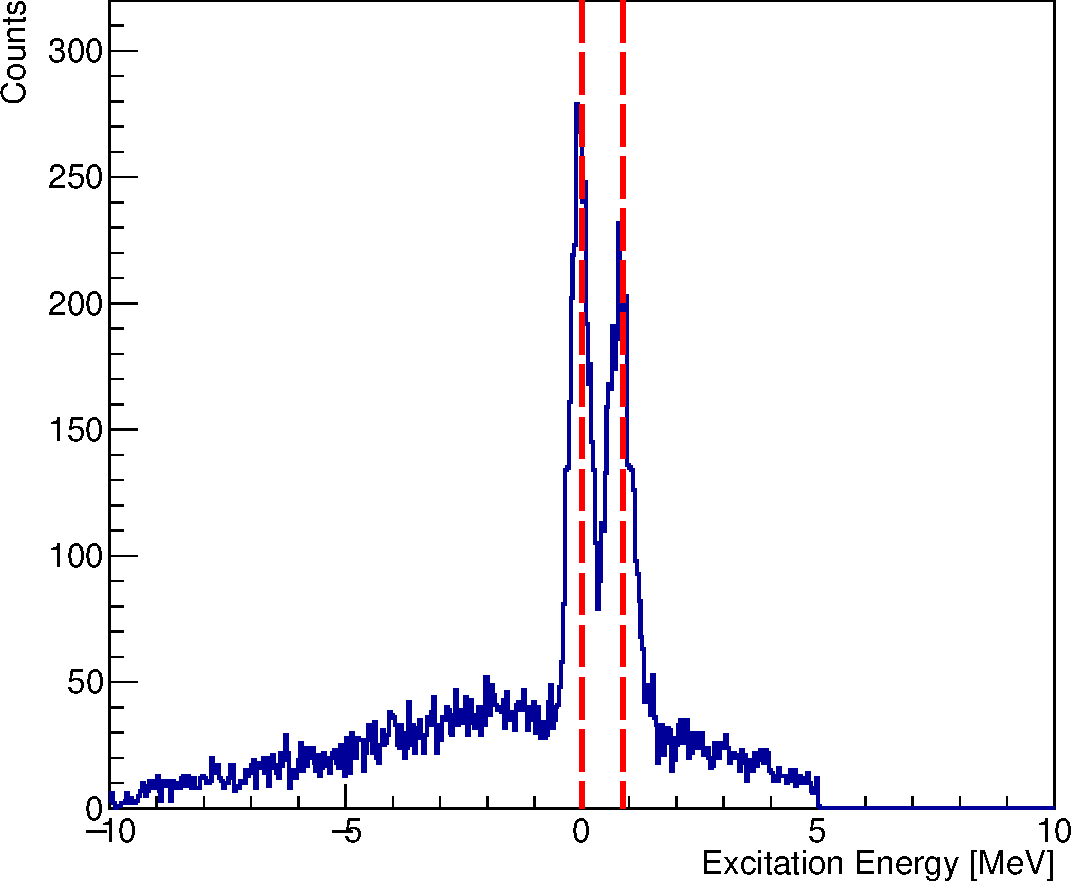
\includegraphics[width=0.9\textwidth]{Ex_1}\\
	\end{column}
	\begin{column}{0.6\textwidth}
		\centering
		\footnotesize Correction to Target thickness computed scanning over different values to match the adopted excitation energies.\\
		 \textbf{Optimal Value} $\rightarrow$ -4.3~$\mu$m~(PRELIMINARY)\\
		
		\vspace{0.05\textheight}
		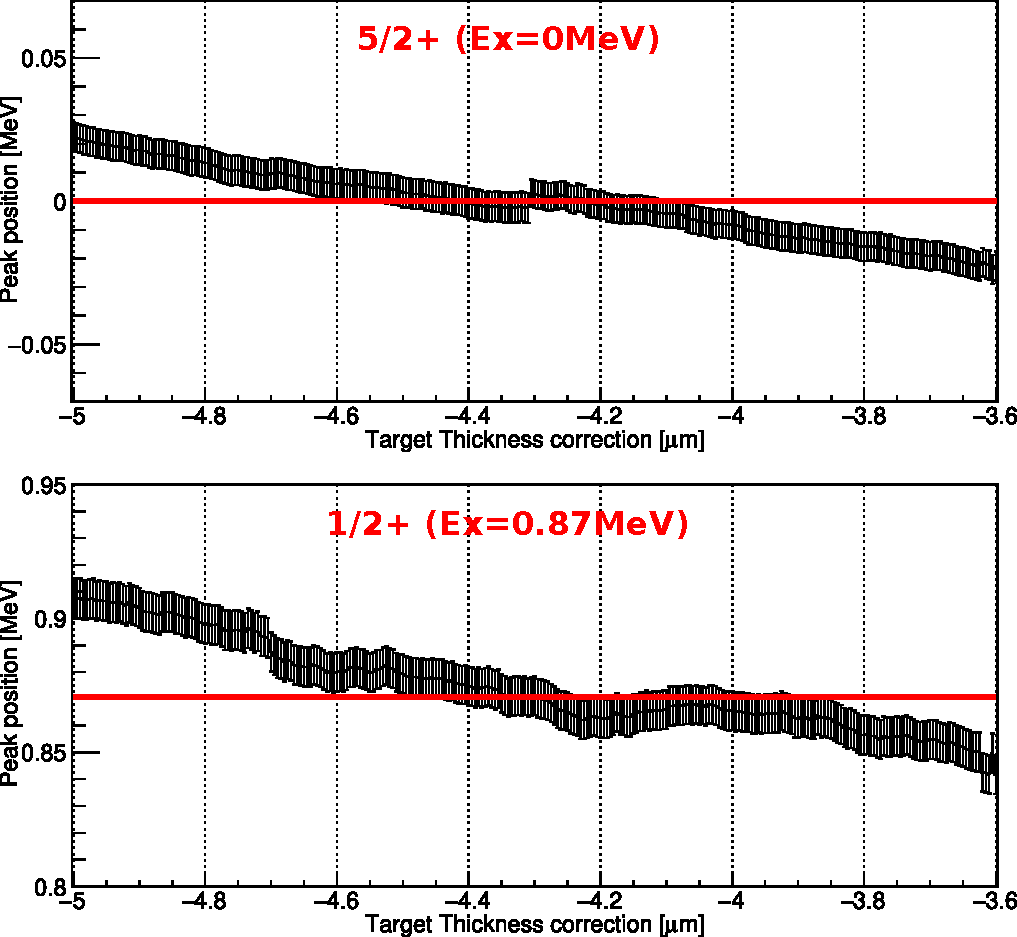
\includegraphics[width=0.9\textwidth]{Thickness_opt_inkscaped}\\
	\end{column}
\end{columns}
\end{frame}

\begin{frame}
\centering
\vspace{0.02\textheight}
\textbf{\Large Angular Distribution}
\vspace{0.01\textheight}
\begin{columns}
	\begin{column}{0.5\textwidth}
		\centering\\
		\vspace{-0.01\textheight}
		\hspace{0.02\textwidth}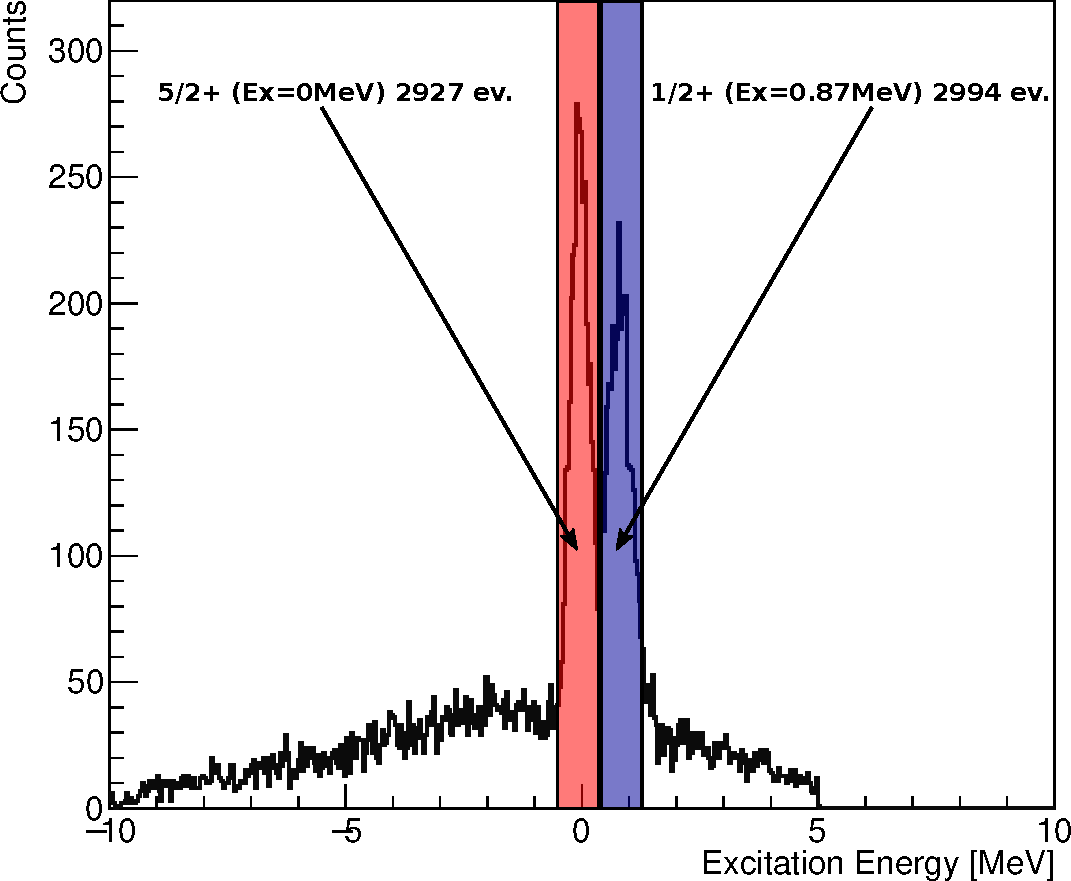
\includegraphics[width=0.75\textwidth]{Ex_2}\\
		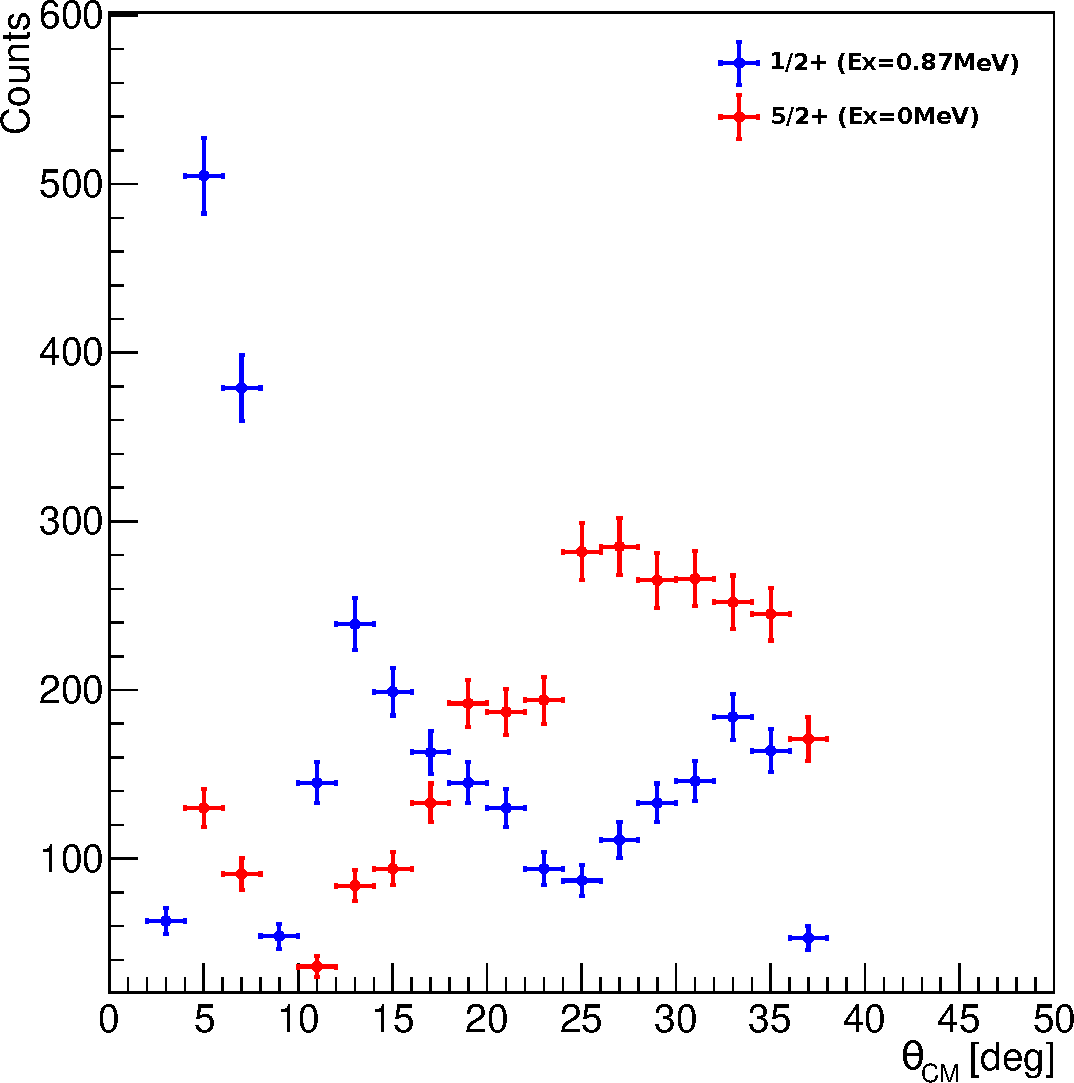
\includegraphics[width=0.73\textwidth]{ARawDist}\\
	\end{column}
	\begin{column}{0.5\textwidth}
		\centering\\
		\footnotesize
		\vspace{-0.04\textheight}
		Normalized with simulated angular efficiency\\
		$\downarrow$\\
		Fit over the theoretical distribution\\
		(Annular efficiency to be checked)
		
		\vspace{0.03\textheight}
		\tiny DWBA calculation from Jesus Casal\\
		INFN Sezione di Padova\\				
		\vspace{0.02\textheight}
		Optical potential from\\ An et al.,PRC 73.5 (2006)\\
		Watson et al., PR 182.4 (1969)\\
		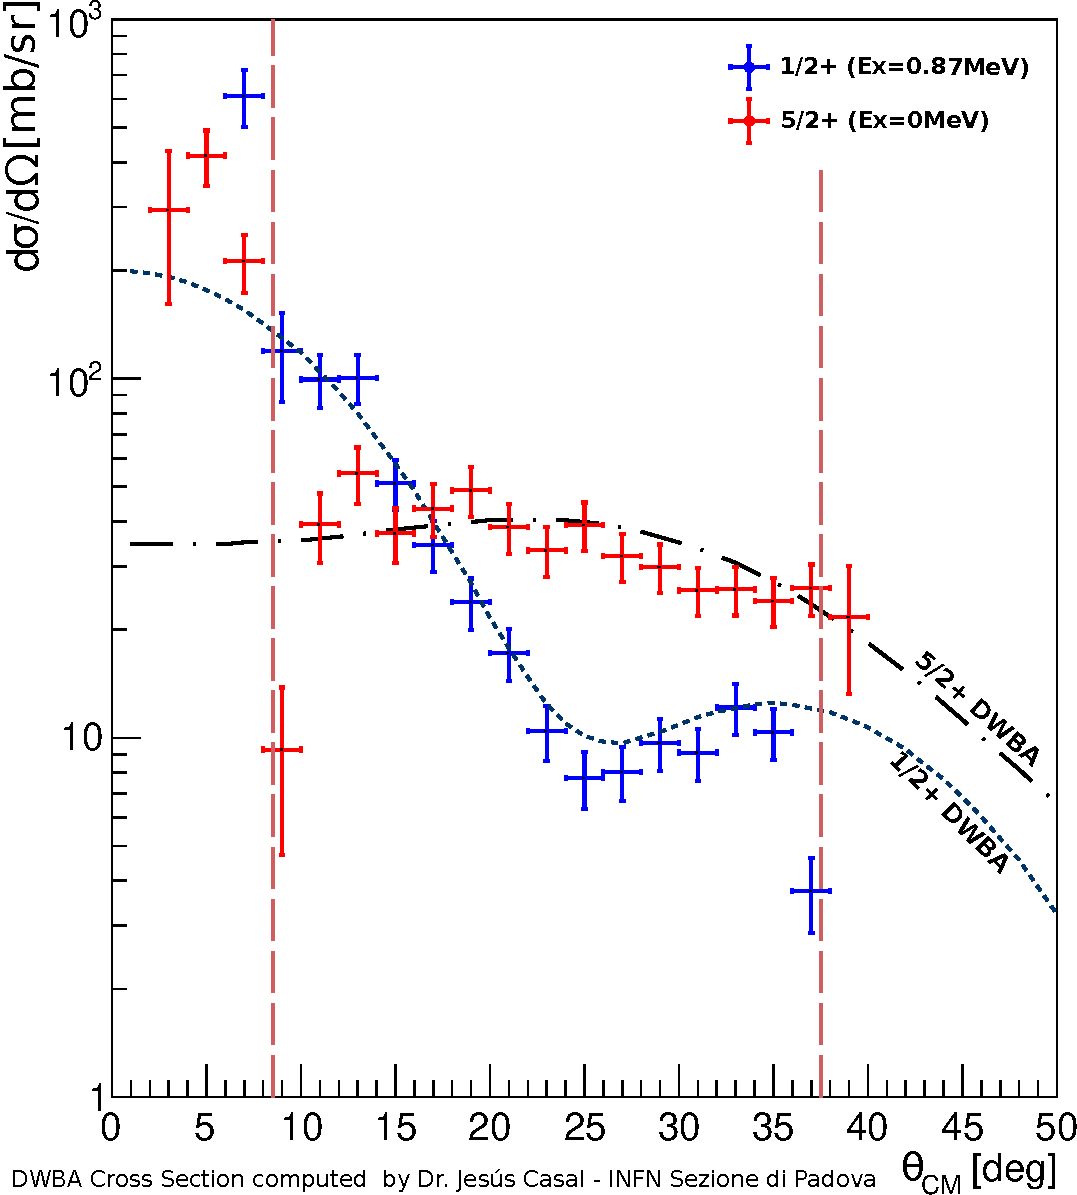
\includegraphics[width=0.7\textwidth]{ADist_jesus}\\

	\end{column}
\end{columns}
\end{frame}

\begin{frame}
\centering
\vspace{0.02\textheight}
\textbf{\Large AGATA}
\vspace{0.01\textheight}
\begin{columns}
	\begin{column}{0.5\textwidth}
		\centering\\
		\vspace{-0.03\textheight}
		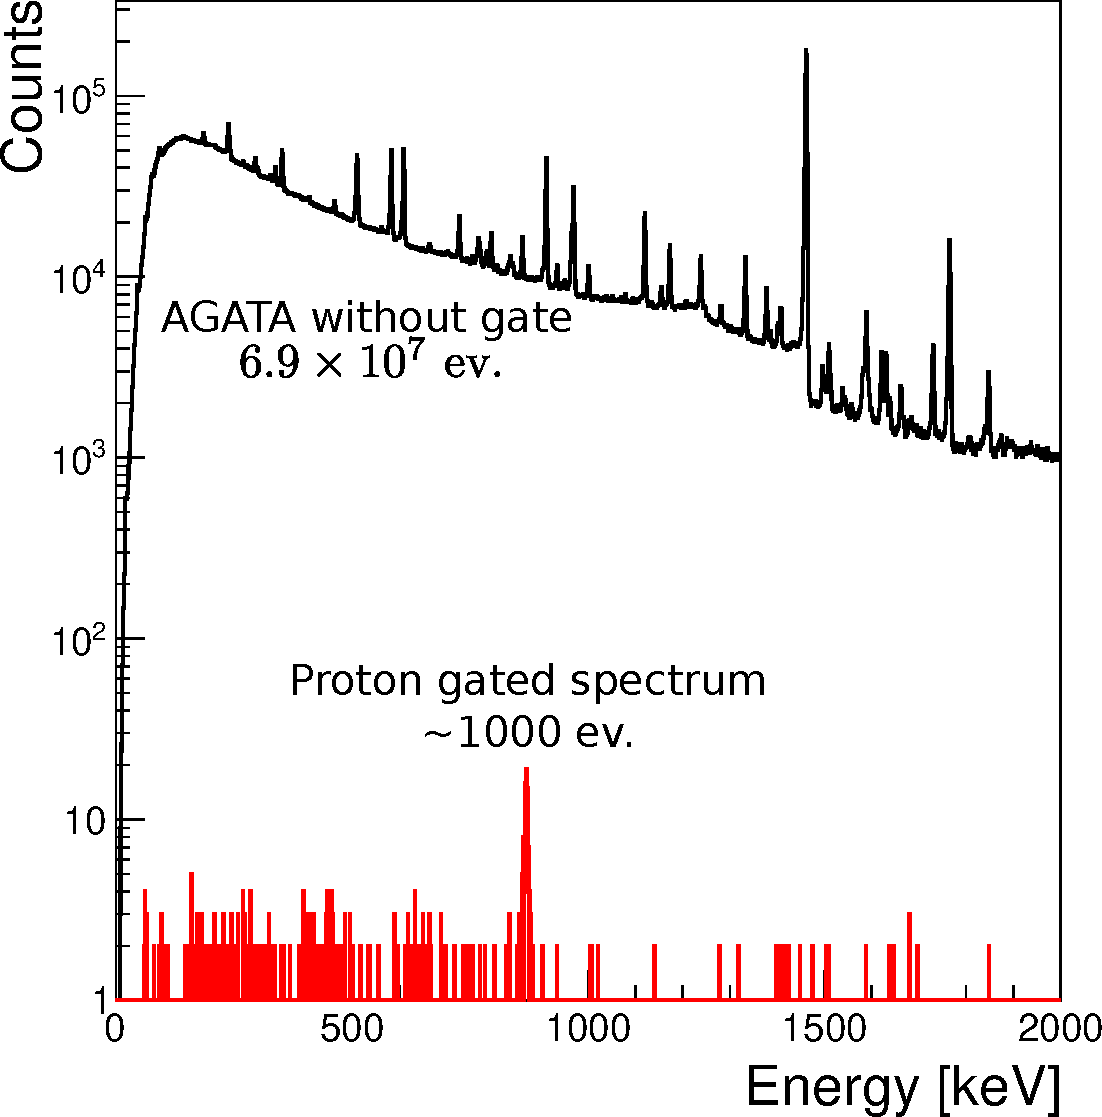
\includegraphics[width=\textwidth]{AGATASpectra}\\
	\end{column}
	\begin{column}{0.5\textwidth}
		\begin{itemize}
    	    		\centering
			\item 870~keV excitation peak integral\\ (background removed)\\ $\downarrow$\\ $2562 \pm 50$~protons
			\item{870~keV gamma peak integral (background removed)\\
					$\downarrow$\\ 
					\vspace{-0.07\textheight}
					\begin{align*}
					\text{\textbf{Add Back}}\ &\rightarrow\ 177\pm 13\ \gamma\\
					\text{\textbf{Tracking}}\ &\rightarrow\ 160\pm 13\ \gamma
					\end{align*}
			  	}
		\end{itemize}
		\centering
		\textbf{Efficiency Estimate:}\\
		\vspace{-0.07\textheight}
		\begin{align*}
	  		\text{\textbf{Add Back}}\ &\rightarrow\ 7.0 \pm 0.5\ \%\\
	 		\text{\textbf{Tracking}}\ &\rightarrow\ 6.3 \pm 0.5\ \%
		\end{align*}
		\footnotesize Tracking performed with standard parameters
	\end{column}
\end{columns}
\end{frame}

%\begin{frame}{Impact Matrix}
%    	\vspace{-0.05\textheight}
%    \begin{overlayarea}{\textwidth}{0.1\textheight}
%	\centering
%	\textbf{11~h. acquisition long at $\mathbf{\sim 4\ 10^{4}}$~pps}
%	%\vspace{0.05\textheight}
%	\end{overlayarea}
%	\begin{columns}
%		\begin{column}{0.5\textwidth}
%			\begin{overlayarea}{\textwidth}{0.5\textheight}
%				\centering
%				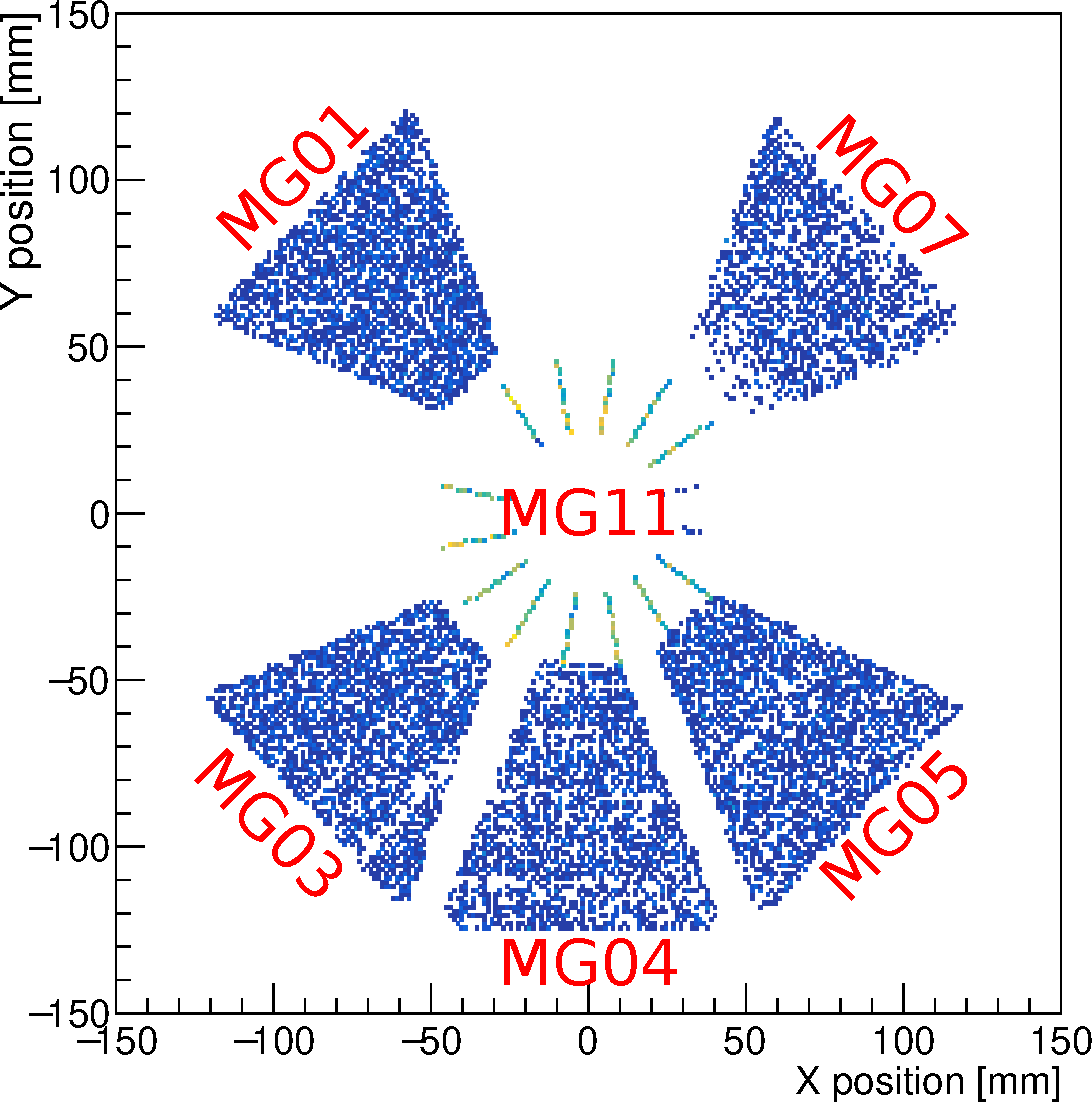
\includegraphics[width=0.5\textwidth]{MGimpact}
%			\end{overlayarea}
%		\end{column}
%		\begin{column}{0.5\textwidth}
%			\begin{overlayarea}{\textwidth}{0.5\textheight}
%				\centering       
%				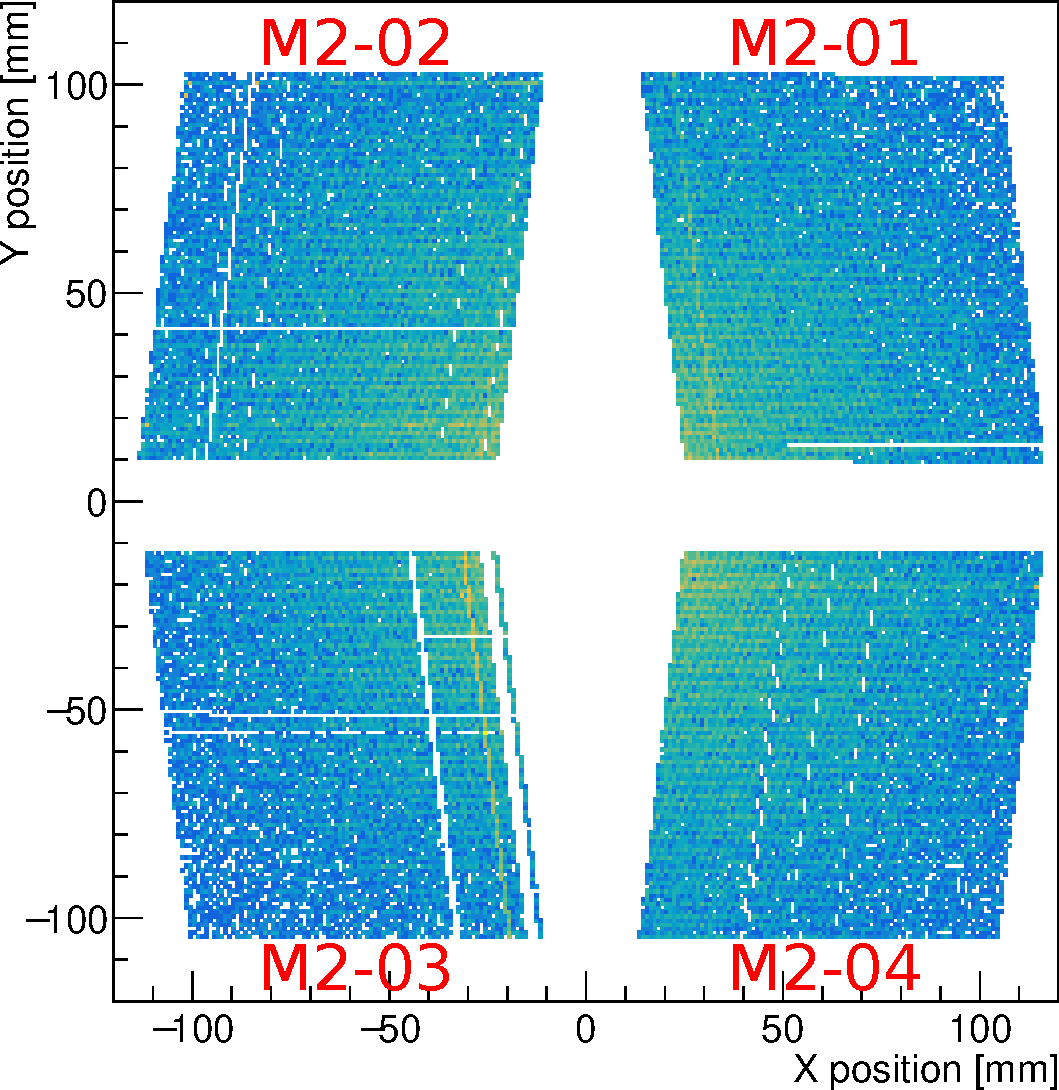
\includegraphics[width=0.5\textwidth]{MMimpact}\\
%		    \end{overlayarea}	
%		\end{column}
%	\end{columns}
%	\centering       
%	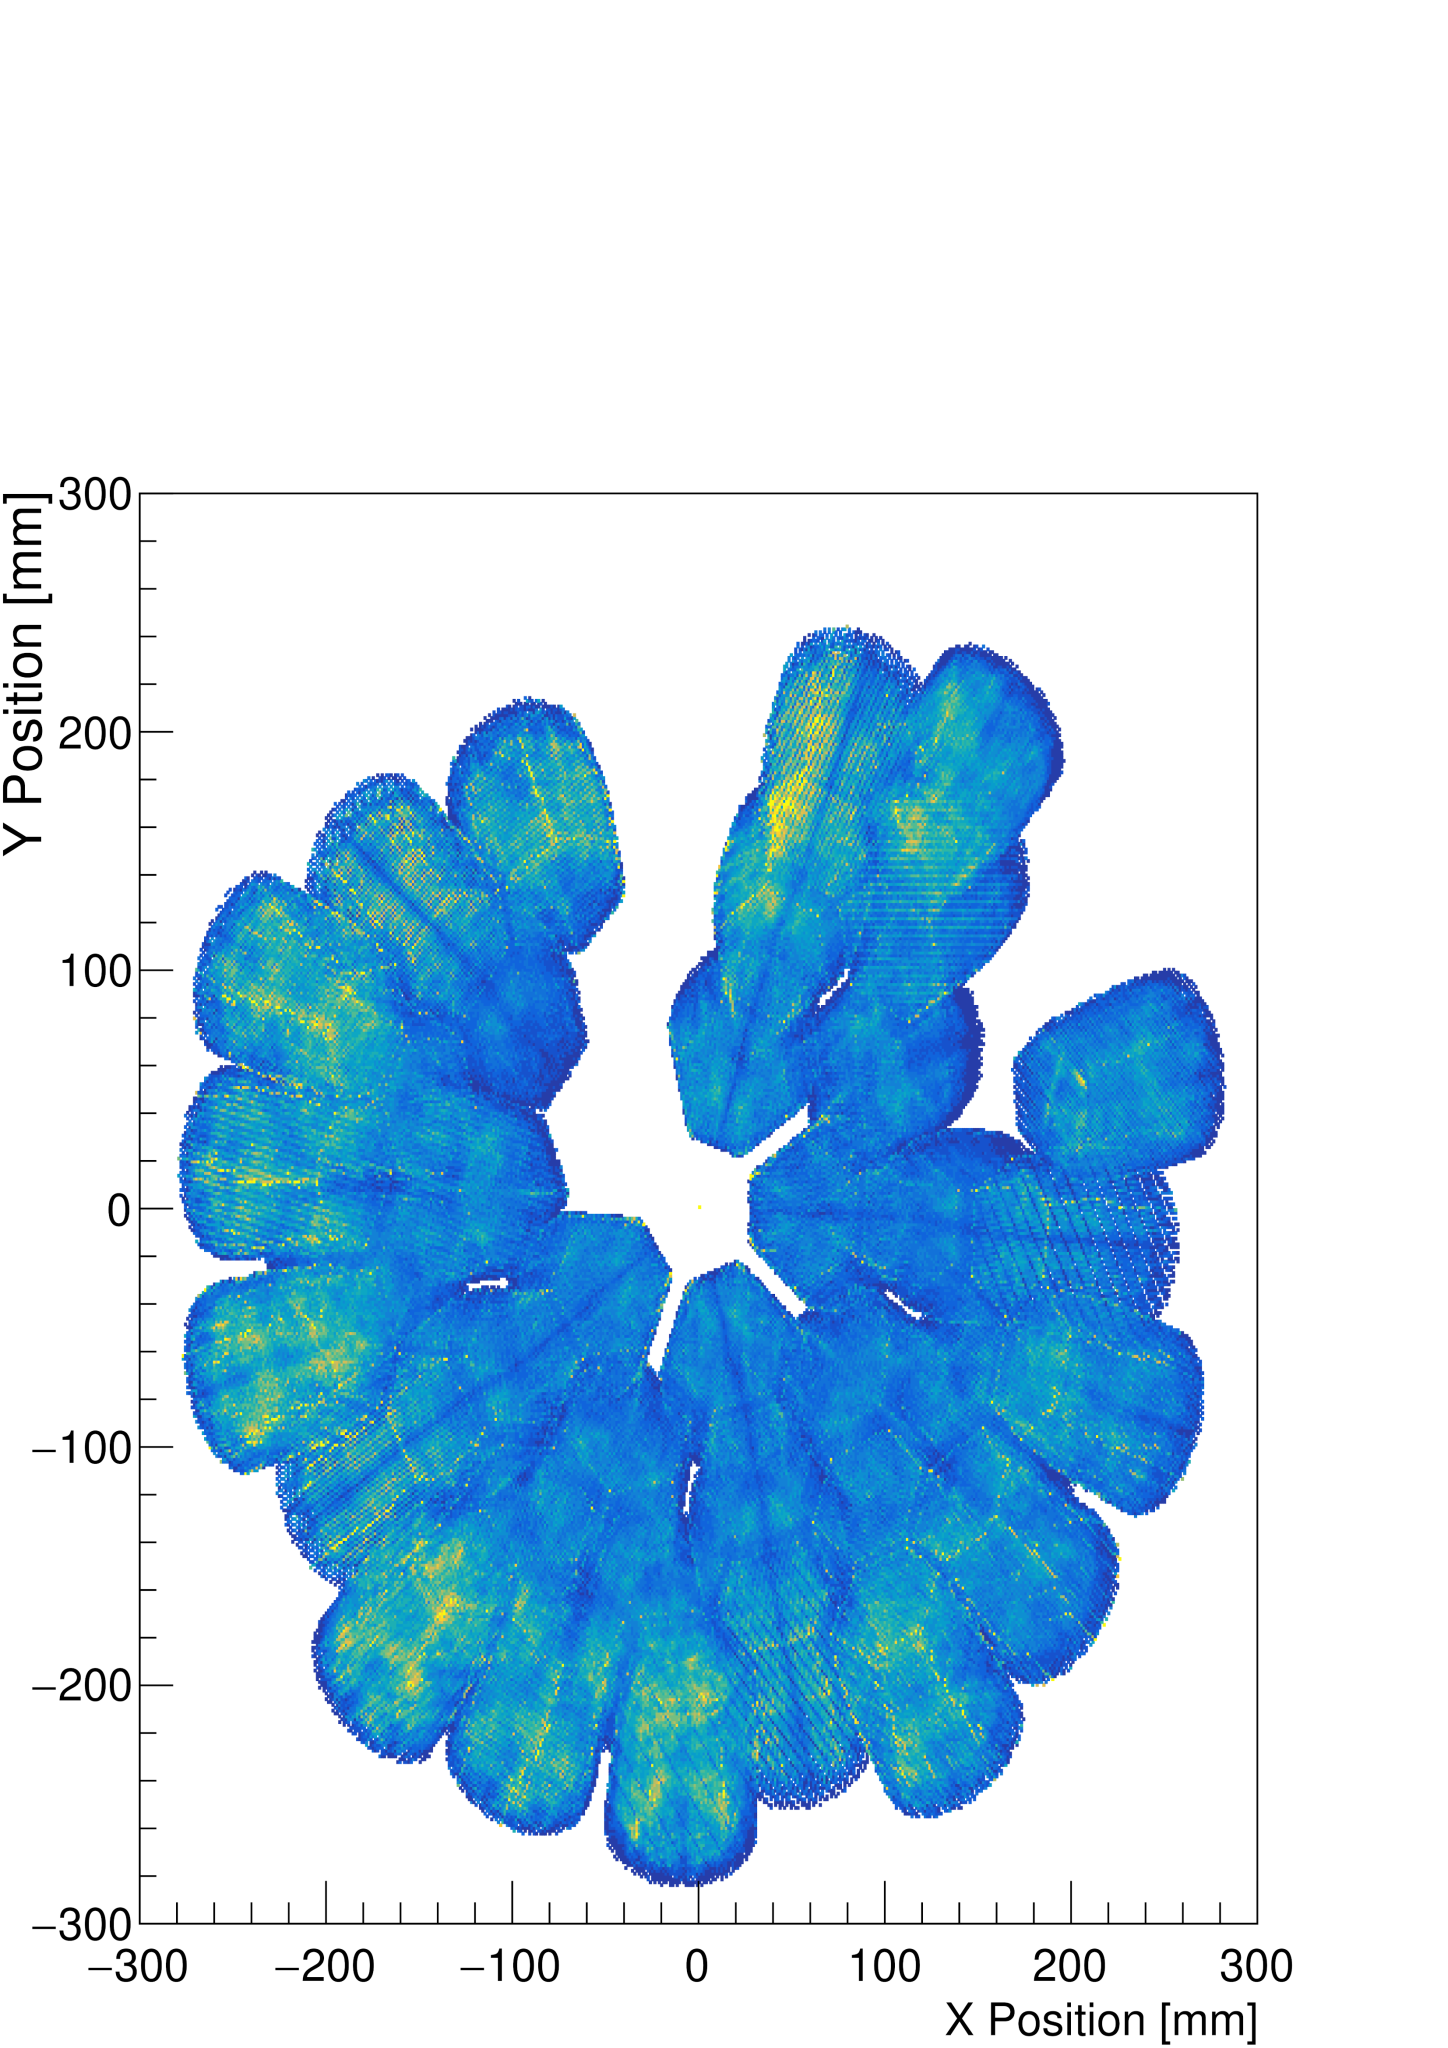
\includegraphics[width=0.5\textwidth]{AGATAimpact}\\
%\end{frame}

\end{document}